\section{Gauß'sche Strahlenoptik}
Wir möchten die Kenngrößen des Laserstrahls in der Gaußoptik bestimmen.
Hierzu wird der Laserstrahl mit einer CCD-Kamera aufgenommen.
\subsection{Herleitung von Gleichung 10 aus Gleichung 4}
Bevor man $M^2$ berechnet, ist zuerst Gleichung (11) aus der Versuchsanleitung herzuleiten.\\
Die Breite eines Laserstrahls lässt sich wie folgt schreiben \citep[vgl.][S. 10]{Anleitung}:
\begin{equation}
    w(z)=w_0\sqrt{1+\left(\frac{\lambda z}{\pi w_0^2}\right)^2}
\end{equation}
Für die reale Ausbreitung eines Laserstrahls folgt:
\begin{equation}
    w(z)=w_0\sqrt{1+\left(M^2\frac{\lambda z}{\pi w_0^2}\right)^2}
\end{equation}
Der Koordinatenursprung $z$ liegt an der engsten Stelle des Strahles, mit $w(0)=w_0=d_0/2$.
Hierbei bezeichnet $d$ den Durchmesser des Strahles. Somit kann man $z$ zu $L_0-L_1$ umschreiben (vgl. \ref{img:skizze}), damit der 'neue' Ursprung nicht mehr am Linsenmittelpunkt liegt.
Die Gleichung wird nach $M^2$ aufgelöst:
\begin{equation}
    M^2=\frac{\pi d_0^2}{2\lambda\left(L_0-L_1\right)}\sqrt{\frac{d_1^2}{d_0^2}-1}
\end{equation}
\begin{figure}[h]
    \centering\includegraphics[width=0.5\textwidth]{Auswertung-Dominik/GaußLaser.jpg}
    \label{img:skizze}
    \caption{Skizze zu den Variablen}
\end{figure}
\subsection{Bestimmung von M$^2$}
Zunächst wird der Durchmesser und die Halbwertsbreite der einzelnen aufgenommenen Strahlen bestimmt.
Hierfür werden die Messdaten nacheinander in GNU-Plot geladen.
Dort wird das Offset von der y-Achse ($y_{off}$) und die Spitze ($y_{max}$) der Gaußkurve bestimmt per Hand jeweils für die x- und y-Richtung bestimmt.
Somit kann man die Hälfte der Höhe wie folgt berechnen:
\begin{equation}
    y_{half}=\frac{y_{max}-y_{off}}{2}+y_{off}
\end{equation}
Dort wird eine Gerade eingezeichnet und die Breite zwischen den Schnittpunkten mit der Gaußkurve ist die Halbwertsbreite (FWHM).
Dabei wurde darauf geachtet, dass (vor allem bei den ersten Messungen) die Gaußkurve etwas extrapoliert werden musste, um die Werte zu bestimmen.
Der Durchmesser ($d$) wurde als Intervall zwischen den Schnittpunkten mit $y_{off}$ gemessen.
Mit alles Messungen erhält man für den Praktikumslaser:
\begin{table}[h]
    \centering
      \begin{tabular}{cc|cccc}
      Position (cm)& Graufilter & FWHM x (mm) & FWHM y (mm) & $d_x$ (mm) & $d_y$ (mm) \\\hline
      3 & 4 & 1,16 & 1,09 & 2,6 & 2,74 \\
      10 & 4 & 0,92 & 0,88 & 2,2 & 2,18 \\
      15 & 4,3 & 0,78 & 0,74 & 1,87 & 2,74 \\
      20 & 4,3 & 0,63 & 0,56 & 1,56 & 1,48 \\
      25 & 4,6 & 0,41 & 0,45 & 1,2 & 0,57 \\
      30 & 5 & 0,3 & 0,29 & 0,77 & 0,7 \\
      35 & 5,3 & 0,17 & 0,16 & 0,54 & 0,5 \\
      36 & 5,3 & 0,16 & 0,13 & 0,46 & 0,45 \\
      37 & 5,3 & 0,14 & 0,12 & 0,42 & 0,38 \\
      38 & 5,3 & 0,12 & 0,11 & 0,35 & 0,29 \\
      39 & 5,9 & 0,12 & 0,11 & 0,32 & 0,28 \\
      40 & 5,9 & 0,11 & 0,1 & 0,31 & 0,27 \\
      41 & 5,9 & 0,1 & 0,1 & 0,25 & 0,25 \\
      42 & 5,9 & 0,09 & 0,09 & 0,27 & 0,28 \\
      43 & 5,9 & 0,11 & 0,11 & 0,3 & 0,31 \\
      44 & 5,9 & 0,13 & 0,14 & 0,37 & 0,37 \\
      45 & 5,9 & 0,16 & 0,16 & 0,43 & 0,41 \\
      50 & 5 & 0,33 & 0,35 & 0,75 & 0,75 \\
      55 & 4,6 & 0,44 & 0,49 & 1,02 & 1,04 \\
      60 & 4,6 & 0,57 & 0,55 & 1,13 & 1,26 \\
      \end{tabular}
      \caption{Halbwertsbreiten des Praktikumslasers}
  \end{table}
  \begin{figure}[h]
    \scalebox{0.9}{% GNUPLOT: LaTeX picture with Postscript
\begingroup
  % Encoding inside the plot.  In the header of your document, this encoding
  % should to defined, e.g., by using
  % \usepackage[cp1252,<other encodings>]{inputenc}
  \inputencoding{cp1252}%
  \makeatletter
  \providecommand\color[2][]{%
    \GenericError{(gnuplot) \space\space\space\@spaces}{%
      Package color not loaded in conjunction with
      terminal option `colourtext'%
    }{See the gnuplot documentation for explanation.%
    }{Either use 'blacktext' in gnuplot or load the package
      color.sty in LaTeX.}%
    \renewcommand\color[2][]{}%
  }%
  \providecommand\includegraphics[2][]{%
    \GenericError{(gnuplot) \space\space\space\@spaces}{%
      Package graphicx or graphics not loaded%
    }{See the gnuplot documentation for explanation.%
    }{The gnuplot epslatex terminal needs graphicx.sty or graphics.sty.}%
    \renewcommand\includegraphics[2][]{}%
  }%
  \providecommand\rotatebox[2]{#2}%
  \@ifundefined{ifGPcolor}{%
    \newif\ifGPcolor
    \GPcolorfalse
  }{}%
  \@ifundefined{ifGPblacktext}{%
    \newif\ifGPblacktext
    \GPblacktexttrue
  }{}%
  % define a \g@addto@macro without @ in the name:
  \let\gplgaddtomacro\g@addto@macro
  % define empty templates for all commands taking text:
  \gdef\gplbacktext{}%
  \gdef\gplfronttext{}%
  \makeatother
  \ifGPblacktext
    % no textcolor at all
    \def\colorrgb#1{}%
    \def\colorgray#1{}%
  \else
    % gray or color?
    \ifGPcolor
      \def\colorrgb#1{\color[rgb]{#1}}%
      \def\colorgray#1{\color[gray]{#1}}%
      \expandafter\def\csname LTw\endcsname{\color{white}}%
      \expandafter\def\csname LTb\endcsname{\color{black}}%
      \expandafter\def\csname LTa\endcsname{\color{black}}%
      \expandafter\def\csname LT0\endcsname{\color[rgb]{1,0,0}}%
      \expandafter\def\csname LT1\endcsname{\color[rgb]{0,1,0}}%
      \expandafter\def\csname LT2\endcsname{\color[rgb]{0,0,1}}%
      \expandafter\def\csname LT3\endcsname{\color[rgb]{1,0,1}}%
      \expandafter\def\csname LT4\endcsname{\color[rgb]{0,1,1}}%
      \expandafter\def\csname LT5\endcsname{\color[rgb]{1,1,0}}%
      \expandafter\def\csname LT6\endcsname{\color[rgb]{0,0,0}}%
      \expandafter\def\csname LT7\endcsname{\color[rgb]{1,0.3,0}}%
      \expandafter\def\csname LT8\endcsname{\color[rgb]{0.5,0.5,0.5}}%
    \else
      % gray
      \def\colorrgb#1{\color{black}}%
      \def\colorgray#1{\color[gray]{#1}}%
      \expandafter\def\csname LTw\endcsname{\color{white}}%
      \expandafter\def\csname LTb\endcsname{\color{black}}%
      \expandafter\def\csname LTa\endcsname{\color{black}}%
      \expandafter\def\csname LT0\endcsname{\color{black}}%
      \expandafter\def\csname LT1\endcsname{\color{black}}%
      \expandafter\def\csname LT2\endcsname{\color{black}}%
      \expandafter\def\csname LT3\endcsname{\color{black}}%
      \expandafter\def\csname LT4\endcsname{\color{black}}%
      \expandafter\def\csname LT5\endcsname{\color{black}}%
      \expandafter\def\csname LT6\endcsname{\color{black}}%
      \expandafter\def\csname LT7\endcsname{\color{black}}%
      \expandafter\def\csname LT8\endcsname{\color{black}}%
    \fi
  \fi
    \setlength{\unitlength}{0.0500bp}%
    \ifx\gptboxheight\undefined%
      \newlength{\gptboxheight}%
      \newlength{\gptboxwidth}%
      \newsavebox{\gptboxtext}%
    \fi%
    \setlength{\fboxrule}{0.5pt}%
    \setlength{\fboxsep}{1pt}%
\begin{picture}(7200.00,5040.00)%
    \gplgaddtomacro\gplbacktext{%
      \csname LTb\endcsname%%
      \put(814,704){\makebox(0,0)[r]{\strut{}$0$}}%
      \put(814,1390){\makebox(0,0)[r]{\strut{}$0.5$}}%
      \put(814,2076){\makebox(0,0)[r]{\strut{}$1$}}%
      \put(814,2762){\makebox(0,0)[r]{\strut{}$1.5$}}%
      \put(814,3447){\makebox(0,0)[r]{\strut{}$2$}}%
      \put(814,4133){\makebox(0,0)[r]{\strut{}$2.5$}}%
      \put(814,4819){\makebox(0,0)[r]{\strut{}$3$}}%
      \put(946,484){\makebox(0,0){\strut{}$0$}}%
      \put(1922,484){\makebox(0,0){\strut{}$10$}}%
      \put(2898,484){\makebox(0,0){\strut{}$20$}}%
      \put(3875,484){\makebox(0,0){\strut{}$30$}}%
      \put(4851,484){\makebox(0,0){\strut{}$40$}}%
      \put(5827,484){\makebox(0,0){\strut{}$50$}}%
      \put(6803,484){\makebox(0,0){\strut{}$60$}}%
    }%
    \gplgaddtomacro\gplfronttext{%
      \csname LTb\endcsname%%
      \put(209,2761){\rotatebox{-270}{\makebox(0,0){\strut{}Durchmesser des Strahls (mm)}}}%
      \put(3874,154){\makebox(0,0){\strut{}Abstand von Linse (cm)}}%
      \csname LTb\endcsname%%
      \put(5816,4646){\makebox(0,0)[r]{\strut{}x-Durchmesser}}%
      \csname LTb\endcsname%%
      \put(5816,4426){\makebox(0,0)[r]{\strut{}y-Durchmesser}}%
    }%
    \gplgaddtomacro\gplbacktext{%
      \csname LTb\endcsname%%
      \put(814,704){\makebox(0,0)[r]{\strut{}$0$}}%
      \put(814,1390){\makebox(0,0)[r]{\strut{}$0.5$}}%
      \put(814,2076){\makebox(0,0)[r]{\strut{}$1$}}%
      \put(814,2762){\makebox(0,0)[r]{\strut{}$1.5$}}%
      \put(814,3447){\makebox(0,0)[r]{\strut{}$2$}}%
      \put(814,4133){\makebox(0,0)[r]{\strut{}$2.5$}}%
      \put(814,4819){\makebox(0,0)[r]{\strut{}$3$}}%
      \put(946,484){\makebox(0,0){\strut{}$0$}}%
      \put(1922,484){\makebox(0,0){\strut{}$10$}}%
      \put(2898,484){\makebox(0,0){\strut{}$20$}}%
      \put(3875,484){\makebox(0,0){\strut{}$30$}}%
      \put(4851,484){\makebox(0,0){\strut{}$40$}}%
      \put(5827,484){\makebox(0,0){\strut{}$50$}}%
      \put(6803,484){\makebox(0,0){\strut{}$60$}}%
    }%
    \gplgaddtomacro\gplfronttext{%
      \csname LTb\endcsname%%
      \put(209,2761){\rotatebox{-270}{\makebox(0,0){\strut{}Durchmesser des Strahls (mm)}}}%
      \put(3874,154){\makebox(0,0){\strut{}Abstand von Linse (cm)}}%
      \csname LTb\endcsname%%
      \put(5816,4646){\makebox(0,0)[r]{\strut{}x-Durchmesser}}%
      \csname LTb\endcsname%%
      \put(5816,4426){\makebox(0,0)[r]{\strut{}y-Durchmesser}}%
    }%
    \gplbacktext
    \put(0,0){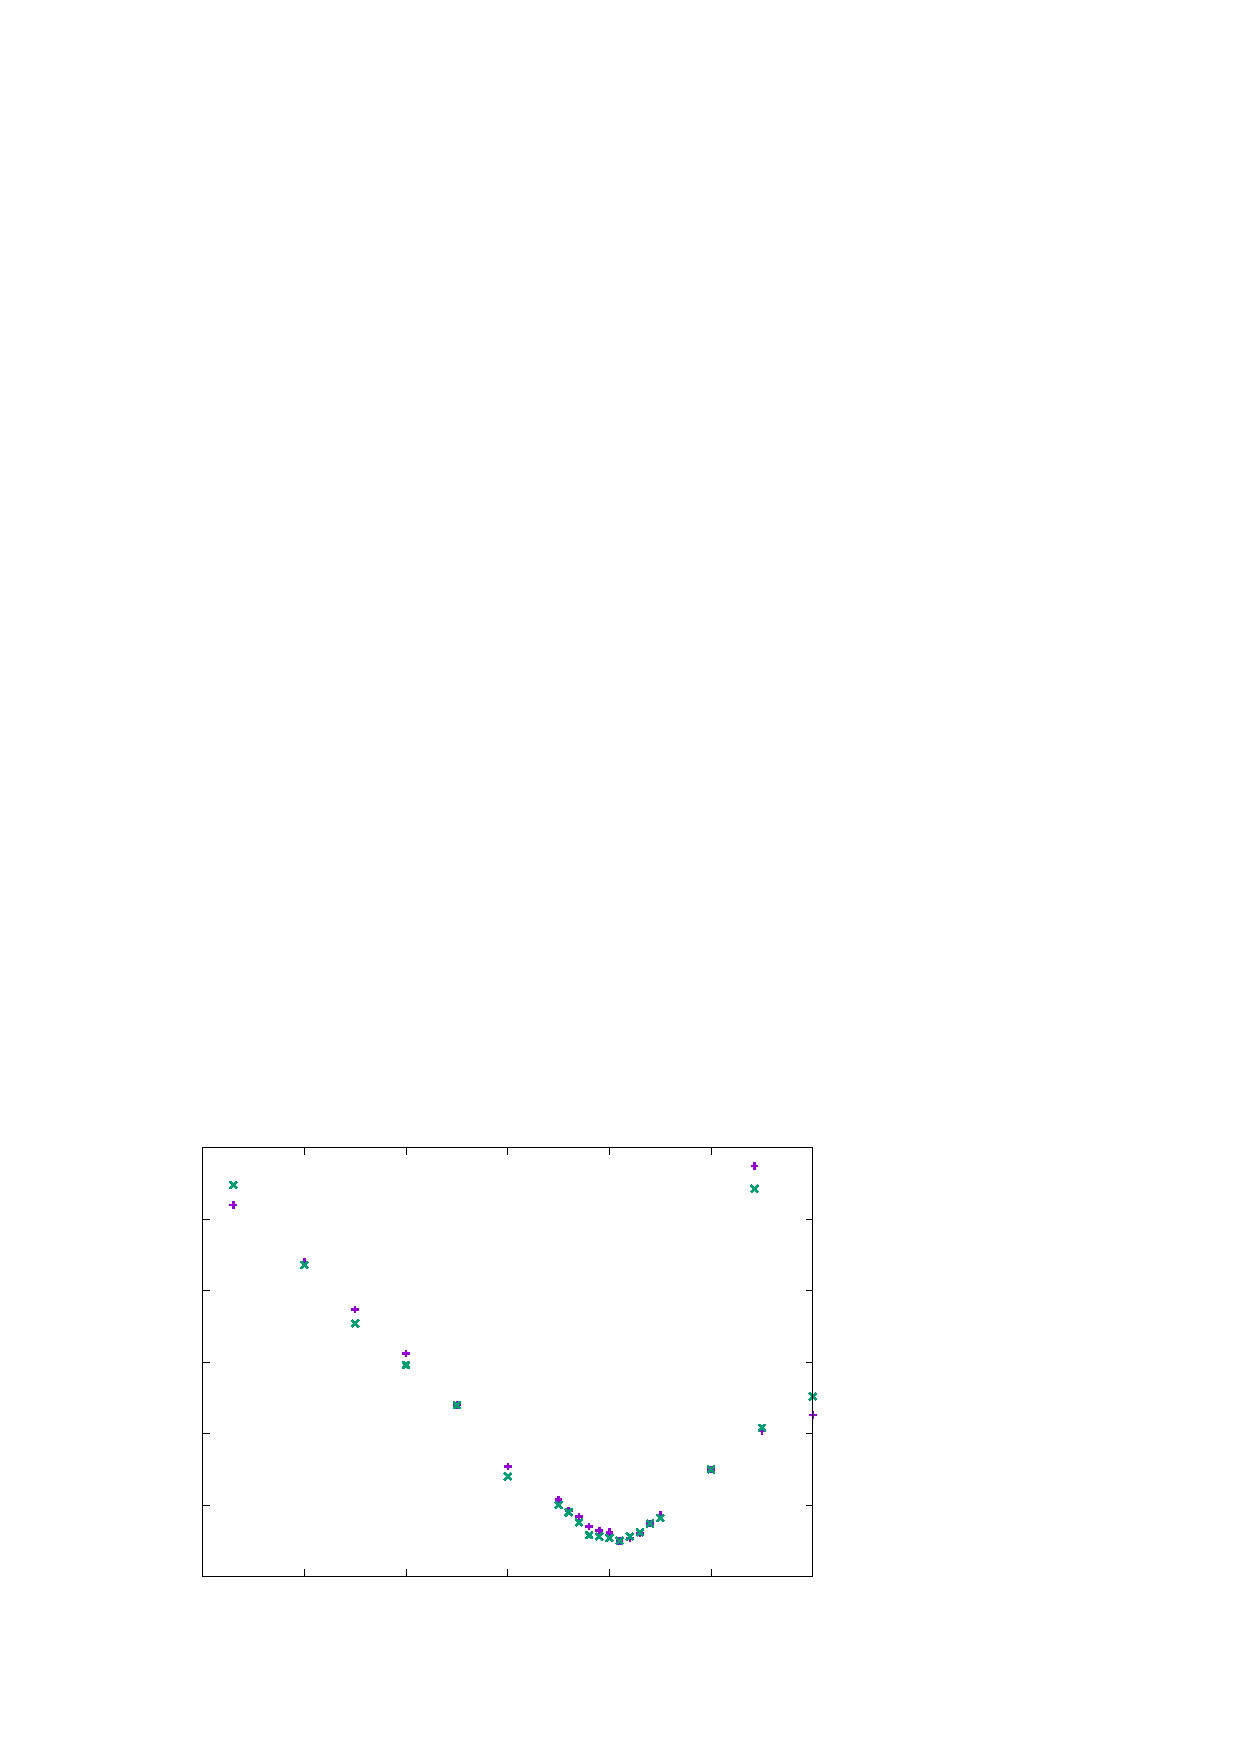
\includegraphics[width={360.00bp},height={252.00bp}]{Auswertung-Dominik/exp2}}%
    \gplfronttext
  \end{picture}%
\endgroup
}
    \centering\caption{Durchmesser des Praktikumslasers}
  \end{figure}\newpage
Und für den Hilfslaser:
\begin{table}[h]
    \centering
      \begin{tabular}{cc|cccc}
        Position (cm)& Graufilter & FWHM x (mm) & FWHM y (mm) & $d_x$ (mm) & $d_y$ (mm) \\\hline
      3 & 3,6 & 0,95 & 0,86 & 2,31 & 2,04 \\
      10 & 4 & 0,81 & 0,8 & 1,96 & 1,77 \\
      15 & 4 & 0,69 & 0,64 & 1,6 & 1,45 \\
      20 & 4,3 & 0,55 & 0,54 & 1,27 & 1,19 \\
      25 & 4,6 & 0,4 & 0,37 & 0,88 & 0,84 \\
      30 & 5 & 0,24 & 0,22 & 0,54 & 0,51 \\
      31 & 5,3 & 0,21 & 0,2 & 0,49 & 0,46 \\
      32 & 5,3 & 0,18 & 0,17 & 0,45 & 0,43 \\
      33 & 5,3 & 0,15 & 0,14 & 0,39 & 0,35 \\
      34 & 5,6 & 0,14 & 0,13 & 0,38 & 0,35 \\
      35 & 5,6 & 0,11 & 0,1 & 0,34 & 0,27 \\
      36 & 5,6 & 0,1 & 0,1 & 0,27 & 0,27 \\
      37 & 5,6 & 0,11 & 0,11 & 0,3 & 0,32 \\
      38 & 5,6 & 0,12 & 0,12 & 0,32 & 0,29 \\
      39 & 5,6 & 0,13 & 0,13 & 0,39 & 0,31 \\
      40 & 5,3 & 0,14 & 0,14 & 0,4 & 0,35 \\
      45 & 5 & 0,22 & 0,21 & 0,77 & 0,69 \\
      50 & 4,6 & 0,39 & 0,36 & 1,03 & 0,83 \\
      55 & 4,3 & 0,55 & 0,5 & 1,34 & 1,15 \\
      60 & 4 & 0,64 & 0,63 & 1,57 & 1,6 \\
      \end{tabular}
      \caption{Halbwertsbreiten des Hilfslasers}
  \end{table}
  \begin{figure}[h]
    \centering\scalebox{0.9}{% GNUPLOT: LaTeX picture with Postscript
\begingroup
  % Encoding inside the plot.  In the header of your document, this encoding
  % should to defined, e.g., by using
  % \usepackage[cp1252,<other encodings>]{inputenc}
  \inputencoding{cp1252}%
  \makeatletter
  \providecommand\color[2][]{%
    \GenericError{(gnuplot) \space\space\space\@spaces}{%
      Package color not loaded in conjunction with
      terminal option `colourtext'%
    }{See the gnuplot documentation for explanation.%
    }{Either use 'blacktext' in gnuplot or load the package
      color.sty in LaTeX.}%
    \renewcommand\color[2][]{}%
  }%
  \providecommand\includegraphics[2][]{%
    \GenericError{(gnuplot) \space\space\space\@spaces}{%
      Package graphicx or graphics not loaded%
    }{See the gnuplot documentation for explanation.%
    }{The gnuplot epslatex terminal needs graphicx.sty or graphics.sty.}%
    \renewcommand\includegraphics[2][]{}%
  }%
  \providecommand\rotatebox[2]{#2}%
  \@ifundefined{ifGPcolor}{%
    \newif\ifGPcolor
    \GPcolorfalse
  }{}%
  \@ifundefined{ifGPblacktext}{%
    \newif\ifGPblacktext
    \GPblacktexttrue
  }{}%
  % define a \g@addto@macro without @ in the name:
  \let\gplgaddtomacro\g@addto@macro
  % define empty templates for all commands taking text:
  \gdef\gplbacktext{}%
  \gdef\gplfronttext{}%
  \makeatother
  \ifGPblacktext
    % no textcolor at all
    \def\colorrgb#1{}%
    \def\colorgray#1{}%
  \else
    % gray or color?
    \ifGPcolor
      \def\colorrgb#1{\color[rgb]{#1}}%
      \def\colorgray#1{\color[gray]{#1}}%
      \expandafter\def\csname LTw\endcsname{\color{white}}%
      \expandafter\def\csname LTb\endcsname{\color{black}}%
      \expandafter\def\csname LTa\endcsname{\color{black}}%
      \expandafter\def\csname LT0\endcsname{\color[rgb]{1,0,0}}%
      \expandafter\def\csname LT1\endcsname{\color[rgb]{0,1,0}}%
      \expandafter\def\csname LT2\endcsname{\color[rgb]{0,0,1}}%
      \expandafter\def\csname LT3\endcsname{\color[rgb]{1,0,1}}%
      \expandafter\def\csname LT4\endcsname{\color[rgb]{0,1,1}}%
      \expandafter\def\csname LT5\endcsname{\color[rgb]{1,1,0}}%
      \expandafter\def\csname LT6\endcsname{\color[rgb]{0,0,0}}%
      \expandafter\def\csname LT7\endcsname{\color[rgb]{1,0.3,0}}%
      \expandafter\def\csname LT8\endcsname{\color[rgb]{0.5,0.5,0.5}}%
    \else
      % gray
      \def\colorrgb#1{\color{black}}%
      \def\colorgray#1{\color[gray]{#1}}%
      \expandafter\def\csname LTw\endcsname{\color{white}}%
      \expandafter\def\csname LTb\endcsname{\color{black}}%
      \expandafter\def\csname LTa\endcsname{\color{black}}%
      \expandafter\def\csname LT0\endcsname{\color{black}}%
      \expandafter\def\csname LT1\endcsname{\color{black}}%
      \expandafter\def\csname LT2\endcsname{\color{black}}%
      \expandafter\def\csname LT3\endcsname{\color{black}}%
      \expandafter\def\csname LT4\endcsname{\color{black}}%
      \expandafter\def\csname LT5\endcsname{\color{black}}%
      \expandafter\def\csname LT6\endcsname{\color{black}}%
      \expandafter\def\csname LT7\endcsname{\color{black}}%
      \expandafter\def\csname LT8\endcsname{\color{black}}%
    \fi
  \fi
    \setlength{\unitlength}{0.0500bp}%
    \ifx\gptboxheight\undefined%
      \newlength{\gptboxheight}%
      \newlength{\gptboxwidth}%
      \newsavebox{\gptboxtext}%
    \fi%
    \setlength{\fboxrule}{0.5pt}%
    \setlength{\fboxsep}{1pt}%
\begin{picture}(7200.00,5040.00)%
    \gplgaddtomacro\gplbacktext{%
      \csname LTb\endcsname%%
      \put(814,704){\makebox(0,0)[r]{\strut{}$0$}}%
      \put(814,1390){\makebox(0,0)[r]{\strut{}$0.5$}}%
      \put(814,2076){\makebox(0,0)[r]{\strut{}$1$}}%
      \put(814,2762){\makebox(0,0)[r]{\strut{}$1.5$}}%
      \put(814,3447){\makebox(0,0)[r]{\strut{}$2$}}%
      \put(814,4133){\makebox(0,0)[r]{\strut{}$2.5$}}%
      \put(814,4819){\makebox(0,0)[r]{\strut{}$3$}}%
      \put(946,484){\makebox(0,0){\strut{}$0$}}%
      \put(1922,484){\makebox(0,0){\strut{}$10$}}%
      \put(2898,484){\makebox(0,0){\strut{}$20$}}%
      \put(3875,484){\makebox(0,0){\strut{}$30$}}%
      \put(4851,484){\makebox(0,0){\strut{}$40$}}%
      \put(5827,484){\makebox(0,0){\strut{}$50$}}%
      \put(6803,484){\makebox(0,0){\strut{}$60$}}%
    }%
    \gplgaddtomacro\gplfronttext{%
      \csname LTb\endcsname%%
      \put(209,2761){\rotatebox{-270}{\makebox(0,0){\strut{}Durchmesser des Strahls (mm)}}}%
      \put(3874,154){\makebox(0,0){\strut{}Abstand von Linse (cm)}}%
      \csname LTb\endcsname%%
      \put(5816,4646){\makebox(0,0)[r]{\strut{}x-Durchmesser}}%
      \csname LTb\endcsname%%
      \put(5816,4426){\makebox(0,0)[r]{\strut{}y-Durchmesser}}%
    }%
    \gplbacktext
    \put(0,0){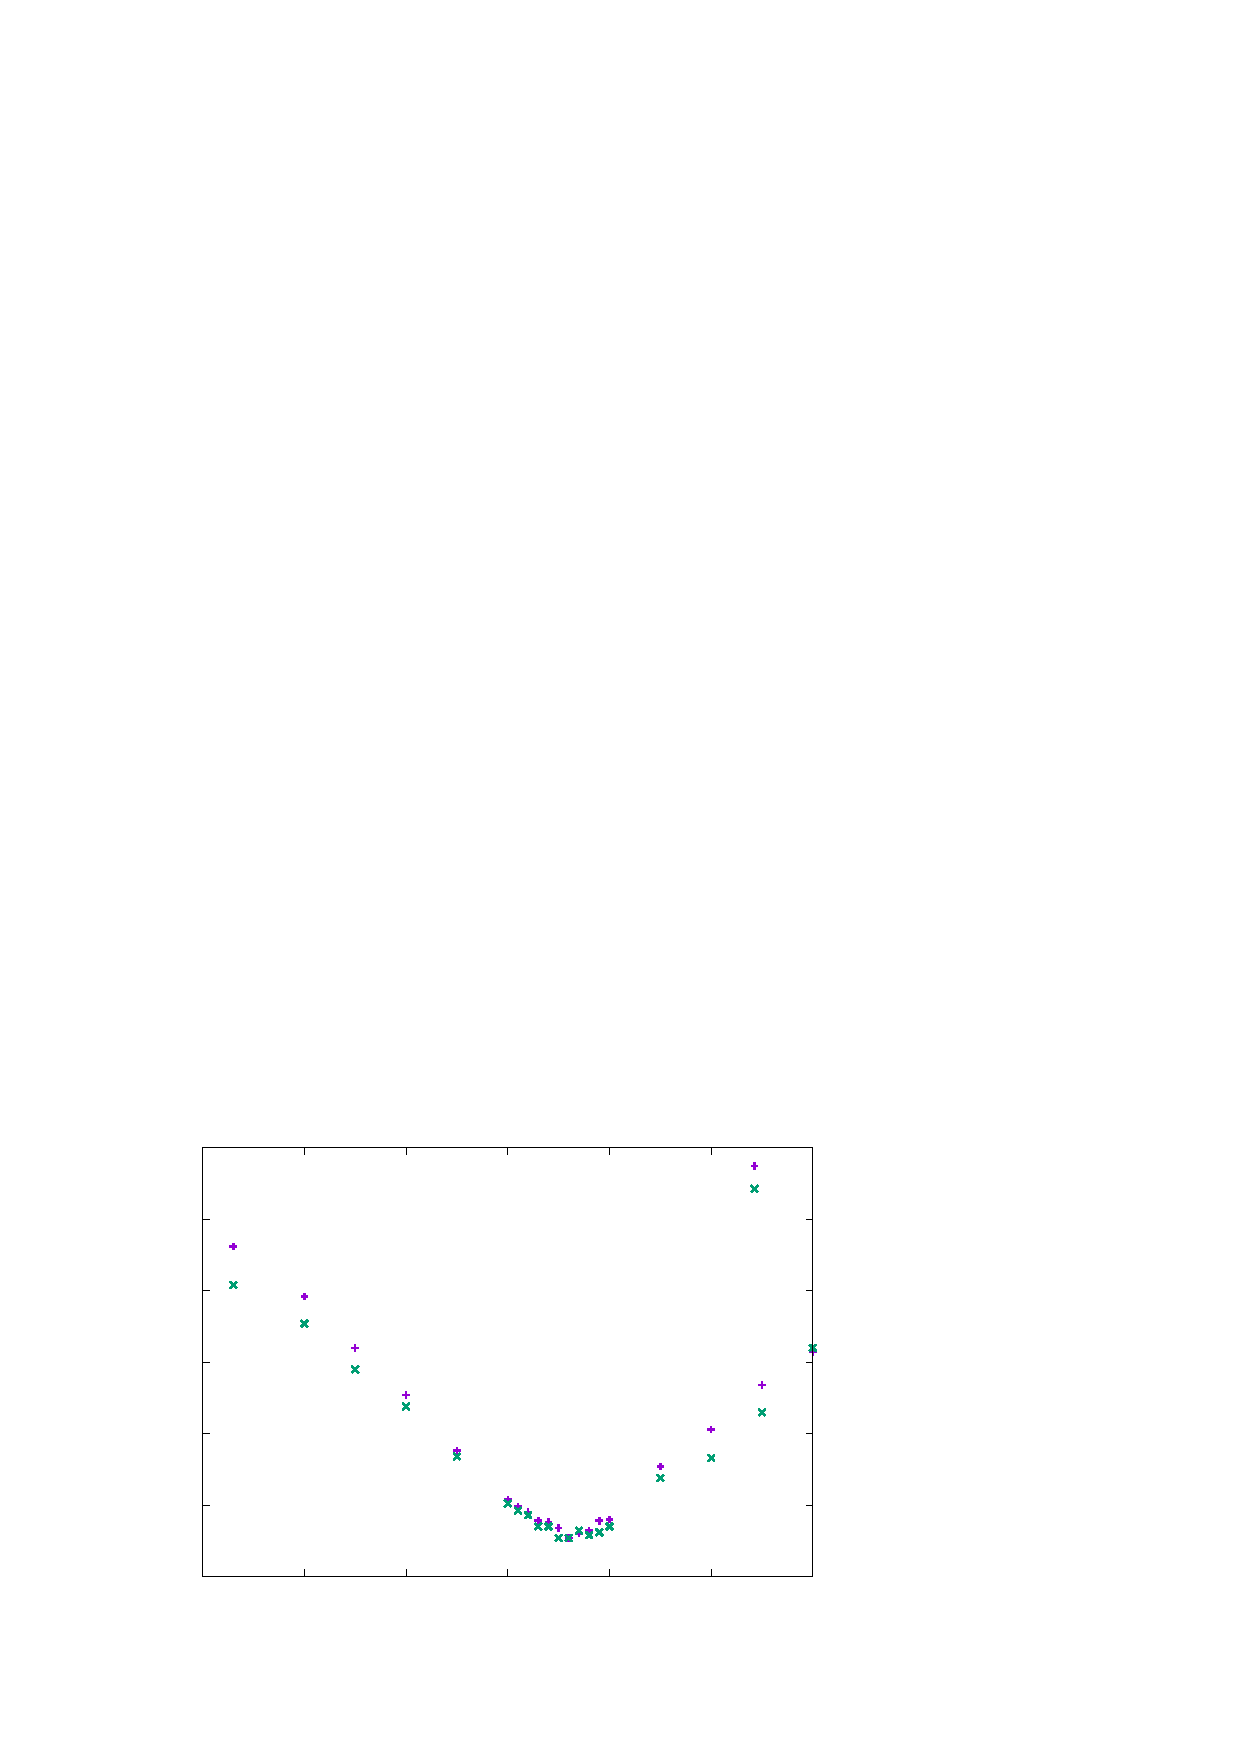
\includegraphics[width={360.00bp},height={252.00bp}]{Auswertung-Dominik/hilf2}}%
    \gplfronttext
  \end{picture}%
\endgroup
}
    \caption{Durchmesser des Hilfslasers}
  \end{figure}\\
Nun kann man $M^2$ für die beiden Laser bestimmen, anschließend wird über alle Werte gemittelt.
\subsubsection{Hilfslaser}
Beim Hilfslaser ist der Abstand des minimalen Durchmessers $L_{0_x}=36\,\text{cm}$ bei horizontaler und $L_{0_y}=36\,\text{cm}$ bei vertikaler Schwingrichtung.
Somit folgt:
\begin{table}[h]
    \centering
    \begin{tabular}{c|ccc}
        &$M^2$ & $L_0$ (cm) & $w_0$ (mm) \\\hline
        horizontal &$\left(6,09\pm4,92\right)$&$\left(36\pm1\right)$&$\left(0,135\pm0,005\right)$\\
        vertikal&$\left(4,99\pm3,62\right)$ &$\left(36\pm1\right)$&$\left(0,135\pm0,005\right)$
    \end{tabular}
    \caption{$M^2$ für den Hilfslaser}
\end{table}
\subsubsection{Praktikumslaser}
Beim Praktikumslaser ist der Abstand des minimalen Durchmessers $L_{0_x}=41\,\text{cm}$ bei horizontaler und $L_{0_y}=41\,\text{cm}$ bei vertikaler Schwingrichtung.
Somit folgt:
\begin{table}[h]
    \centering
    \begin{tabular}{c|ccc}
        &$M^2$ & $L_0$ (cm) & $w_0$ (mm) \\\hline
        horizontal &$\left(5,22\pm2,54\right)$&$\left(41\pm1\right)$&$\left(0,125\pm0,005\right)$\\
        vertikal&$\left(4,73\pm1,66\right)$ &$\left(41\pm1\right)$&$\left(0,125\pm0,005\right)$
    \end{tabular}
    \caption{$M^2$ für den Praktikumslaser}
\end{table}\\
Für beide Laser wurde der Fehler der Länge $L_0$ jeweils mit $1\,\text{cm}$ abgeschätzt, da die genaue Position des Chips in der CCD-Kamera nicht bekannt ist.
Die Länge ist immer die Strecke von Linse zu Kameralinse.\\
Im Vergleich vom Hilfslaser zum Praktikumslaser sieht man, dass dieser eine stärkere Abweichung von Gaußprofil aufweist, da sein $M^2$-Faktor größer ist.
Des Weiteren sind die bestimmten Faktor und deren Fehler sehr groß, was an der Art und Weise der Bestimmung liegen könnte.
\subsection{Brennweite der Linse}
Zur Berechnung der effektiven Brennweite der Linse, wird die abgewandelte Form der Linsengleichung verwendet \citep[vgl.][]{Anleitung}:
\begin{equation}
    \frac{1}{s+\frac{z_R^2}{s-f}}+\frac{1}{s'}=\frac{1}{f}
\end{equation}
Hierbei werden jeweils 2 Minima der Strahlentaille angenommen. Das eine Minimum befindet sich in der Mitte des Resonators und das andere bei $L_0$ hinter der Linse.\\
Wird nun nach f umgestellt, folgt:
\begin{equation}
    f=\frac{s^2+z_R^2+2ss'\pm\sqrt{s^4+z_R^4+2s^2z_R^2-4(s')^2z_R^2}}{2(s'+s)}
\end{equation}
Faktor $z_R$ ist ebenfalls bekannt:
\begin{equation}
    z_R=\frac{\pi w_0^2}{\lambda}
\end{equation}
Somit kann, mit dem im vorangegangenen Kapitel bestimmten $L_0$, die effektive Brennweite der Linse berechnet werden.
Der Fehler wurde über das Fehlerfortpflanzungsgesetz bestimmt:
\begin{equation}
    f=\left(283,9\pm5,8\right)\,\text{mm}
\end{equation}
Wir sehen die effektive Brennweite der Linse, stimmt in etwa mit der angegebenen Brennweite der Linse ($300\,\text{mm}$) überein.
\subsection{Berechnung minimale Strahlentaille}
Nun wollen wir die minimale Strahlentaille berechnen.
Dafür kennen wir die Resonatorlänge $L=\left(545\pm2\right)\,\text{mm}$ und den Krümmungsradius der Spiegel $R=500\,\text{mm}$.
Wir verwenden die Formel:
\begin{equation}
    w_{00}=\sqrt{\frac{\lambda}{2\pi}\cdot\sqrt{L(2R-L)}}
\end{equation}
Somit folgt für die minimale Strahltaille im Resonator:
\begin{equation}
    w_{00}=\left(0,22390\pm0,00004\right)\,\text{mm}
\end{equation}
\subsection{Berechnung des Taillenradius hinter der Linse}
Die theoretische Strahlentaille hinter der Linse lässt sich wie folgt bestimmen:
\begin{equation}
    w_0=\left(\frac{1}{w_{00}^2}\left(1-\frac{s}{f}\right)^2+\frac{1}{f^2}\left(\frac{\pi\cdot w_{00}}{\lambda}\right)^2\right)^{-\frac{1}{2}}
\end{equation}
Somit folgt für die Taille des Versuchslasers:
\begin{equation}
    w_0=\left(0,23\pm0,02\right)\,\text{mm}
\end{equation}
Dieser Wert liegt in der Größenordnung der gemessenen Strahltaille.
Die gemessene Strahlentaille liegt nicht direkt innerhalb der Fehlertoleranz. 
Mögliche Gründe hierfür könnten eine ungenaue Justage des Aufbaus oder das die Gaußkurven falsch abgeschätzt wurden.
\subsection{Laserleistungsdichte}
Wir wollen nun die Leistung pro Fläche im Fokus berechnen.
Hierzu berechnen wir die Fläche (Kreis mit Radius $w_0$), welche im Fokus vom Laser bestrahlt wird.
Die Laserleistung soll nun im Mittel etwa $1\,\text{mW}$ betragen.\\
Bei einem Gaußprofil ist im Bereich der Taille nur $1-1/e^2$-Prozent der gesamt Leistung.
Somit folgt für die Leistung pro Fläche im Fokus:
\begin{equation}
    \frac{P}{A}=\frac{(1-\frac{1}{e^2})\cdot P_{max}}{w_0^2\pi}
\end{equation}
Somit hat der Laser folgende mittlere Leistung pro Fläche:
\begin{equation}
    \frac{P}{A}=\left(1,76\pm0,07\right)\,\frac{\text{W}}{\text{cm}^2}
\end{equation}
Nehmen wir nun für den Laser die von uns gemessene Leistung an, bekommen wir folgende Leistung pro Fläche im Fokus:
\begin{equation}
    \frac{P}{A}=\left(7,6\pm0,2\right)\,\frac{\text{W}}{\text{cm}^2}
\end{equation}
